\documentclass[11pt, oneside]{book}

%%%%%%%%%%%%%%Include Packages%%%%%%%%%%%%%%%%%%%%%%%%%%
\usepackage{xcolor}
\usepackage{mathtools}
\usepackage[a4paper, total={6in, 8in}, margin=1.25in]{geometry}
\usepackage{amsmath}
\usepackage{amssymb}
\usepackage{paralist}
\usepackage{rsfso}
\usepackage{amsthm}
\usepackage{wasysym}
\usepackage[inline]{enumitem}   
\usepackage{hyperref}
\usepackage{tocloft}
\usepackage{wrapfig}
\usepackage{titlesec}
\usepackage{colortbl}
\usepackage{stackengine} 
\usepackage{listings}
%%%%%%%%%%%%%%%%%%%%%%%%%%%%%%%%%%%%%%%%%%%%%%%%%%%%%%%%



%%%%%%%%%%%%%%%Code%%%%%%%%%%%%%%%%%%%%%%%%%%%%%%%%%%%%%
\definecolor{codegreen}{rgb}{0,0.6,0}
\definecolor{codegray}{rgb}{0.5,0.5,0.5}
\definecolor{codepurple}{rgb}{0.58,0,0.82}
\definecolor{backcolour}{rgb}{0.95,0.95,0.92}

\lstdefinestyle{mystyle}{
    backgroundcolor=\color{backcolour},   
    commentstyle=\color{codegreen},
    keywordstyle=\color{magenta},
    numberstyle=\tiny\color{codegray},
    stringstyle=\color{codepurple},
    basicstyle=\ttfamily\footnotesize,
    breakatwhitespace=false,         
    breaklines=true,                 
    captionpos=b,                    
    keepspaces=true,                 
    numbers=left,                    
    numbersep=5pt,                  
    showspaces=false,                
    showstringspaces=false,
    showtabs=false,                  
    tabsize=2
}
%%%%%%%%%%%%%%%%%%%%%%%%%%%%%%%%%%%%%%%%%%%%%%%%%%%%%%%%

%%%%%%%%%%%%%%%Chapter Setting%%%%%%%%%%%%%%%%%%%%%%%%%%
\definecolor{gray75}{gray}{0.75}
\newcommand{\hsp}{\hspace{20pt}}
\titleformat{\chapter}[hang]{\Huge\bfseries}{\thechapter\hsp\textcolor{gray75}{$\mid$}\hsp}{0pt}{\Huge\bfseries}
%%%%%%%%%%%%%%%%%%%%%%%%%%%%%%%%%%%%%%%%%%%%%%%%%%%%%%%%

%%%%%%%%%%%%%%%%%Theorem environments%%%%%%%%%%%%%%%%%%%
\newtheoremstyle{break}
  {\topsep}{\topsep}%
  {\itshape}{}%
  {\bfseries}{}%
  {\newline}{}%
\theoremstyle{break}
\theoremstyle{break}
\newtheorem{axiom}{Axiom}
\newtheorem{thm}{Theorem}[section]
\renewcommand{\thethm}{\arabic{section}.\arabic{thm}}
\newtheorem{lem}{Lemma}[thm]
\newtheorem{cor}{Corollary}[thm]
\newtheorem{defn}{Definition}[thm]
\newenvironment{indEnv}[1][Proof]
  {\proof[#1]\leftskip=1cm\rightskip=1cm}
  {\endproof}
%%%%%%%%%%%%%%%%%%%%%%%%%%%%%%%%%%%%%%%%%%%%%%%%%%%%%%


%%%%%%%%%%%%%%%%%%%%%%%Integral%%%%%%%%%%%%%%%%%%%%%%%
\def\upint{\mathchoice%
    {\mkern13mu\overline{\vphantom{\intop}\mkern7mu}\mkern-20mu}%
    {\mkern7mu\overline{\vphantom{\intop}\mkern7mu}\mkern-14mu}%
    {\mkern7mu\overline{\vphantom{\intop}\mkern7mu}\mkern-14mu}%
    {\mkern7mu\overline{\vphantom{\intop}\mkern7mu}\mkern-14mu}%
  \int}
\def\lowint{\mkern3mu\underline{\vphantom{\intop}\mkern7mu}\mkern-10mu\int}
%%%%%%%%%%%%%%%%%%%%%%%%%%%%%%%%%%%%%%%%%%%%%%%%%%%%%%



\newcommand{\R}{\mathbb{R}}
\newcommand{\N}{\mathbb{N}}
\newcommand{\Z}{\mathbb{Z}}
\newcommand{\Q}{\mathbb{Q}}
\newcommand{\C}{\mathbb{C}}
\newcommand{\T}{\mathcal{T}}
\newcommand{\M}{\mathcal{M}}
\newcommand{\Symm}{\text{Symm}}
\newcommand{\Alt}{\text{Alt}}
\newcommand{\Int}{\text{Int}}
\newcommand{\Bd}{\text{Bd}}
\newcommand{\Power}{\mathcal{P}}
\newcommand{\ee}[1]{\cdot 10^{#1}}
\newcommand{\spa}{\text{span}}
\newcommand{\sgn}{\text{sgn}}
\newcommand{\degr}{\text{deg}}
\newcommand{\pd}{\partial}
\newcommand{\that}[1]{\widetilde{#1}}
\newcommand{\lr}[1]{\left(#1\right)}
\newcommand{\vmat}[1]{\begin{vmatrix} #1 \end{vmatrix}}
\newcommand{\bmat}[1]{\begin{bmatrix} #1 \end{bmatrix}}
\newcommand{\pmat}[1]{\begin{pmatrix} #1 \end{pmatrix}}
\newcommand{\rref}{\xrightarrow{\text{row\ reduce}}}
\newcommand{\txtarrow}[1]{\xrightarrow{\text{#1}}}
\newcommand\oast{\stackMath\mathbin{\stackinset{c}{0ex}{c}{0ex}{\ast}{\Circle}}}
\newcommand{\txt}{Wald's \textit{General Relativity}}

\newcommand{\note}{\color{red}Note: \color{black}}
\newcommand{\remark}{\color{blue}Remark: \color{black}}
\newcommand{\example}{\color{green}Example: \color{black}}
\newcommand{\exercise}{\color{green}Exercise: \color{black}}

%%%%%%%%%%%%%%%%%%%%%%Roman Number%%%%%%%%%%%%%%%%%%%%%%%
\makeatletter
\newcommand*{\rom}[1]{\expandafter\@slowromancap\romannumeral #1@}
\makeatother
%%%%%%%%%%%%%%%%%%%%%%%%%%%%%%%%%%%%%%%%%%%%%%%%%%%%%%%%%

%%%%%%%%%%%%%table of contents%%%%%%%%%%%%%%%%%%%%%%%%%%%%
%\setlength{\cftchapindent}{0em}
%\cftsetindents{section}{2em}{3em}
%
%\renewcommand\cfttoctitlefont{\hfill\huge\bfseries}
%\renewcommand\cftaftertoctitle{\hfill\mbox{}}
%
%\setcounter{tocdepth}{2}
%%%%%%%%%%%%%%%%%%%%%%%%%%%%%%%%%%%%%%%%%%%%%%%%%%%%%%%%%%


%%%%%%%%%%%%%%%%%%%%%Footnotes%%%%%%%%%%%%%%%%%%%%%%%%%%%
\newcommand\blfootnote[1]{%
  \begingroup
  \renewcommand\thefootnote{}\footnote{#1}%
  \addtocounter{footnote}{-1}%
  \endgroup
}
%%%%%%%%%%%%%%%%%%%%%%%%%%%%%%%%%%%%%%%%%%%%%%%%%%%%%%%%%

%%%%%%%%%%%%%%%%%%%%%Section%%%%%%%%%%%%%%%%%%%%%%%%%%%%%
\makeatletter
\def\@seccntformat#1{%
  \expandafter\ifx\csname c@#1\endcsname\c@section\else
  \csname the#1\endcsname\quad
  \fi}
\makeatother
%%%%%%%%%%%%%%%%%%%%%%%%%%%%%%%%%%%%%%%%%%%%%%%%%%%%%%%%%

%%%%%%%%%%%%%%%%%%%%%%%%%%%%%%%%%%%Enumerate%%%%%%%%%%%%%%
\makeatletter
% This command ignores the optional argument 
% for itemize and enumerate lists
\newcommand{\inlineitem}[1][]{%
\ifnum\enit@type=\tw@
    {\descriptionlabel{#1}}
  \hspace{\labelsep}%
\else
  \ifnum\enit@type=\z@
       \refstepcounter{\@listctr}\fi
    \quad\@itemlabel\hspace{\labelsep}%
\fi}
\makeatother
\parindent=0pt
%%%%%%%%%%%%%%%%%%%%%%%%%%%%%%%%%%%%%%%%%%%%%%%%%%%%%%%%%%



\begin{document}

	\begin{titlepage}
		\begin{center}
			\vspace*{0.5cm}
			\Huge \color{red}
				\textbf{Homework 1}\\
			\vspace{0.5cm}			
			\Large \color{black}
			Math 542 - Quantum Optics\\
			Professor Alex Kuzmich
			\vspace{1.5cm}

			
\includegraphics[scale=1.15]{hmm.pdf}
			
			
			\vspace{2cm}
			\LARGE
				\textbf{Jinyan Miao}\\
				\hfill\break
				\LARGE Fall 2023\\
			\vspace{1cm}

		\vspace*{\fill}
		\end{center}			
	\end{titlepage}

\chapter{}
Via Eq.\ (2.55) from the textbook, we have
\begin{align}
i\hbar\, \dot{\mathbf{a}}(t) = \frac{\hbar}{2}
\bmat{
-\omega_0 & 2|\Omega_0(t)|\cos(\omega t- \phi(t) )\\
2|\Omega_0 (t) | \cos(\omega t - \phi(t)) & \omega_0 
}\, \mathbf{a}(t)\,,
\end{align}
with the definition
\begin{align*}
\Omega_0 (t) = \frac{-(\mu_z)_{21}\,E_0(t)}{\hbar} = |\Omega_0 (t) | \, e^{i\,\phi(t)}\,.
\end{align*}

%\section{Assume that $\omega=0$ and $\Omega_0 \in \C$}
With the assumption that $\Omega_0 \in \R$ Eq.\ (1.1) becomes
\begin{align*}
i\hbar\, \dot{\mathbf{a}}(t) = \frac{\hbar}{2}
\bmat{
-\omega_0 & 2\Omega_0\cos(\omega t) \\
2\Omega_0\cos(\omega t) & \omega_0 
}\, \mathbf{a}(t)\,.
\end{align*}
Here we denote $m = i\omega_0\hbar/2$, and $c = -i2\Omega_0\cos(\omega t)$. Then we have
\begin{align*}
\dot{\mathbf{a}} = \mathbf{M}\, \mathbf{a}(t) = \bmat{m & c \\ c & -m}\, \mathbf{a}(t)\,.
\end{align*}
%Assuming here $\mathbf{a}(t) = \mathbf{v}e^{\lambda t}$, then the characteristic equation gives
%\begin{align*}
%0 = \det\left(\mathbf{M} - \lambda \mathbb{I}\right) = (m-\lambda)\cdot (-m-\lambda) - c^2 = -m^2+\lambda^2 - c^2\,,
%\end{align*}
%solving we obtain
%\begin{align*}
%\lambda_{\pm} = \pm(m^2 + c^2)^{-1/2}\,,
%\end{align*}
%with the corresponding eigenvectors
%\begin{align*}
%\mathbf{v}_{\pm} = 
%\end{align*}
Here we will solve the system as a function of $t/T$ numerically with initial conditions $a_1(0) = 1$ and $a_2(0) = 0$. \\

\textit{* The amplitude of $a_1(t)$ and $a_2(t)$ are plotted on the next page. \\ 
** The code is attached at the end of this text.\\
*** For simplicity, the assumption that $\hbar = 1$ has been made.}
\newpage
\section{Assume $\omega T = 0$, $\Omega_0 T\in\{0.5, 1,2,10\}$, $\omega_0 T = 5$.}
\begin{center}
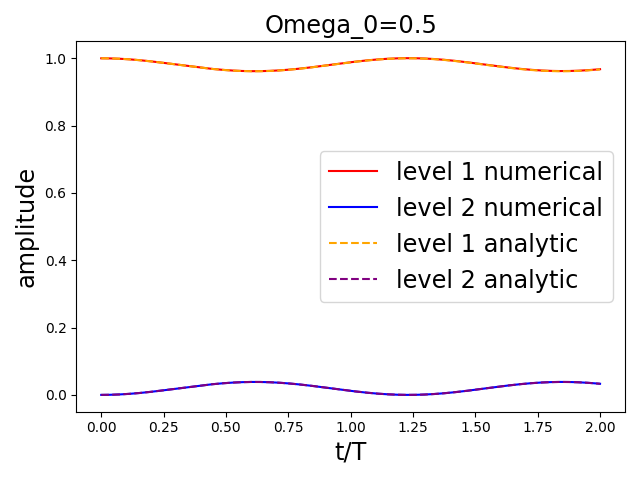
\includegraphics[scale=0.39]{542HW1/a0.5}
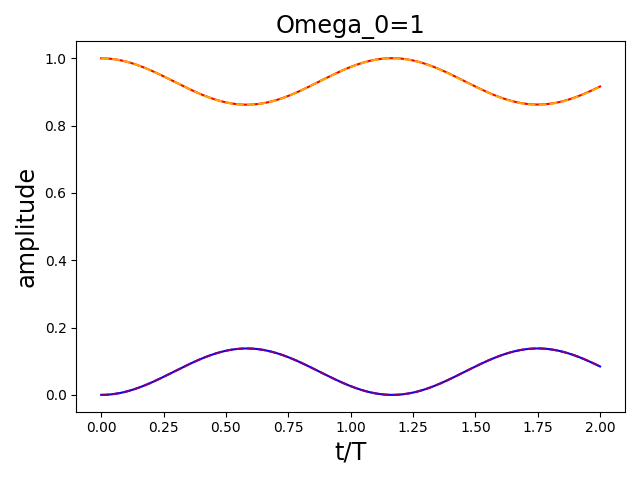
\includegraphics[scale=0.39]{542HW1/a1}\\
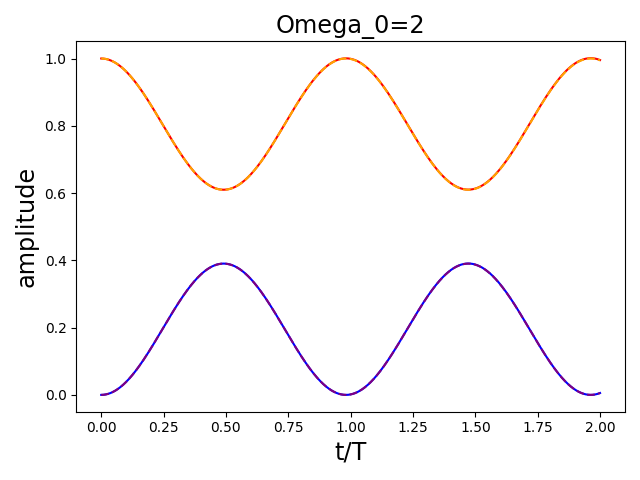
\includegraphics[scale=0.39]{542HW1/a2}
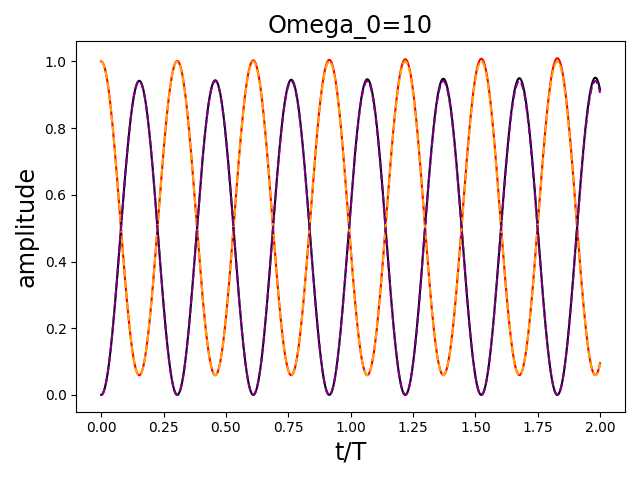
\includegraphics[scale=0.39]{542HW1/a10}\\
\end{center}
\hfill\break
\section{Assume $\omega T = 2$, $\Omega_0 T\in\{0.5, 1,2,10\}$, $\omega_0 T = 0$.}
\begin{center}
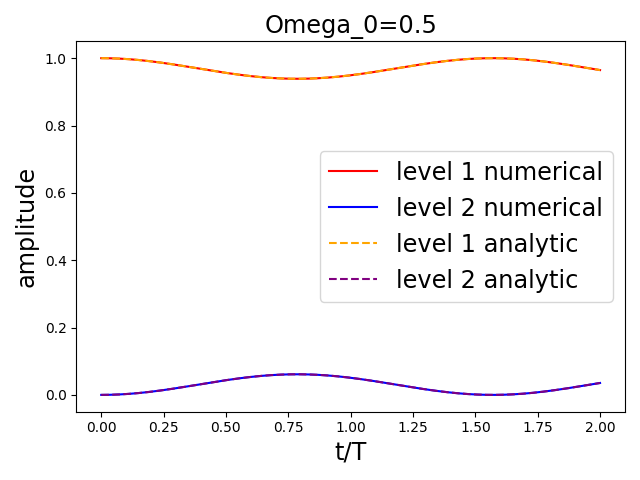
\includegraphics[scale=0.39]{542HW1/b0.5}
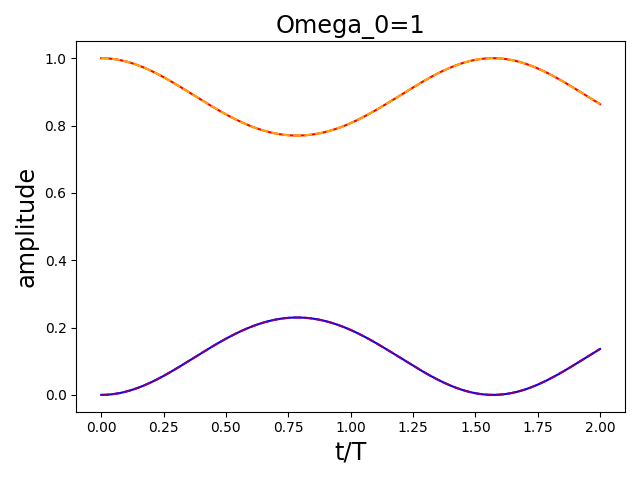
\includegraphics[scale=0.39]{542HW1/b1}\\
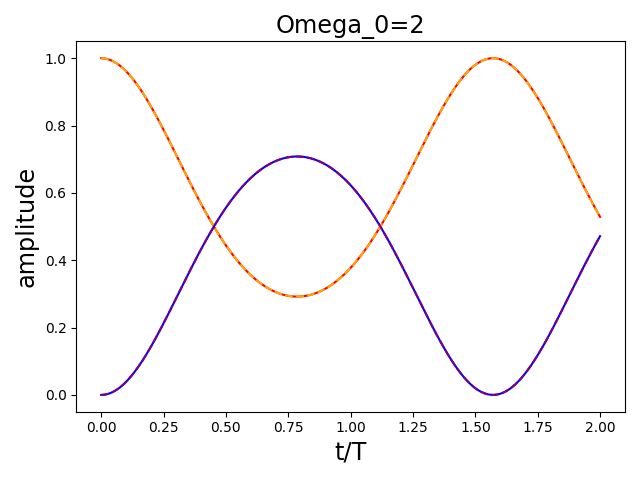
\includegraphics[scale=0.39]{542HW1/b2}
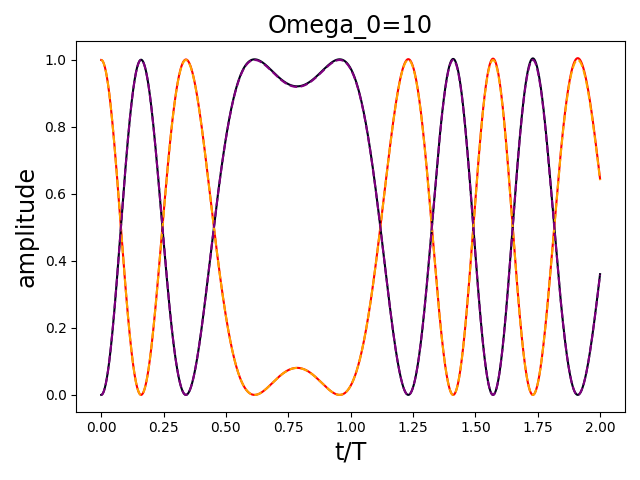
\includegraphics[scale=0.39]{542HW1/b10}\\
\end{center}


\chapter{}
Here we consider the system
\begin{align}
i\hbar \dot{\that{\mathbf{c}}} = \that{\mathbf{H}}\,\that{\mathbf{c}}\,,
\end{align}
where we have
\begin{align*}
\that{\mathbf{H}} = \frac{\hbar}{2}\bmat{-\delta & \Omega_0 \exp(-(t/T)^2) \\ \Omega_0 \exp(-(t/T)^2) &\delta}\,.
\end{align*}
Simplifying (2.1) we obtain
\begin{align}
 \dot{\that{\mathbf{c}}} =
-i \,\bmat{
-\delta/2 & \Omega_0 \exp(-(t/T)^2) /2\\
\Omega_0 \exp(-(t/T)^2)/2 & \delta/2\\
}
\that{\mathbf{c}}\,.
\end{align}
%Defining $E = -i\delta/2$ and $C = -i \Omega_0/2$, we have
%\begin{align*}
%\dot{\that{\mathbf{c}}} =
%\bmat{
%-E & C\exp(-(t/T)^2)\\
%C \exp(-(t/T)^2) & E\\
%} 
%\that{\mathbf{c}}\,.
%\end{align*}
Here Eq. (2.2) agrees with the form of Eq. (2.151) from the textbook, 
\begin{align*}
\dot{\that{\mathbf{c}}}(t) = -i\, \mathbf{A}\, \mathbf{\that{c}}\,. 
\end{align*}
It is not hard to check that the matrix $\mathbf{A}$ has eigenvalues
\begin{align*}
\Lambda_{1,2}(t) = \pm \sqrt{\delta^2 + \Omega_0^2\exp(-2(t/T)^2)}/2 = \pm \Omega(t)/2\,.
\end{align*}
Here we set
\begin{align}
\mathbf{\that{c}} = \mathbf{T}\,\mathbf{x}\,,
\end{align}
where $\mathbf{T}$ diagonalizes $\mathbf{A}$, then via Eq. (2.154) from the text, we have
\begin{align*}
\dot{\mathbf{x}} = -i \mathbf{\Lambda}\, \mathbf{x} - \mathbf{T}^\dagger \dot{\mathbf{T}}\, \mathbf{x}\,,
\end{align*}
where $\mathbf{\Lambda} = \text{diag}(\Lambda_1, \Lambda_2)$. We note further that time-dependent terms in $\mathbf{T}$ can only be in the form of $\sim e^{ t^2/T^2}$, thus all nonzero entries in $\dot{\mathbf{T}}$ involves factor of $1/T^2$. We conclude that entries in $\mathbf{T}^\dagger \dot{\mathbf{T}}$, which have order $1/T^2$, are much less than $|\Lambda_1 - \Lambda_2|\sim \Omega(t)$ because $|\Omega(t) \, T| \gg 1$ by assumption. According to Section 2.7.2 from the textbook, we proceed with the approximation
\begin{align}
\dot{\mathbf{x}} = -i \mathbf{\Lambda}\, \mathbf{x}\,.
\end{align}
Expanding system (2.4), we write
\begin{align*}
\bmat{\dot{x}_1\\\dot{x}_2} = -i\bmat{\sqrt{\delta^2 + \Omega_0^2\exp(-2(t/T)^2)}/2 & 0 \\ 0 & -\sqrt{\delta^2 + \Omega_0^2\exp(-2(t/T)^2)}/2} \bmat{x_1 \\ x_2}\,.
\end{align*}
That is, 
\begin{align*}
\dot{x}_1 = -i\frac{\sqrt{\delta^2 + \Omega_0^2\exp(-2(t/T)^2)}}{2}\, x_1\,,\qquad
\dot{x}_2 = i\frac{\sqrt{\delta^2 + \Omega_0^2\exp(-2(t/T)^2)}}{2}\, x_2\,,
\end{align*}
Solving we obtain
\begin{align}
x_1(t) &=x_1(t_0)\, \exp\left(-i \int_{t_0}^t \frac{\sqrt{\delta^2 + \Omega_0^2\exp(-2(t'/T)^2)}}{2}\, dt'\right)\,,\\
x_2(t) &=x_2(t_0)\, \exp\left(i \int_{t_0}^t \frac{\sqrt{\delta^2 + \Omega_0^2\exp(-2(t'/T)^2)}}{2}\, dt'\right)\,.
\end{align}
A computation through Mathematica finds that we have
\begin{align*}
\mathbf{T} = 
\bmat{
\cos(\theta) & -\sin(\theta)\\
\sin(\theta) & \cos(\theta)
}
\end{align*}
where we have
\begin{align*}
\sin(\theta)  = \sqrt{\frac{1}{2}\left( 1- \frac{\delta}{\Omega}\right)} \,,\qquad
\cos(\theta) = \sqrt{\frac{1}{2}\left( 1 + \frac{\delta}{\Omega}\right)}\,,\qquad
\text{with }\Omega = \sqrt{\delta^2 + \Omega_0^2\,\exp(-2(t/T)^2)}\,.
\end{align*}
Recall from (2.3), we obtain the result
\begin{align*}
\that{c}_1 = x_1\,\cos(\theta) - x_2 \, \sin(\theta)\,,\qquad
\that{c}_2 = x_1\,\sin(\theta) + x_2 \, \cos(\theta)\,.
\end{align*}
In the limit that $\delta(t) \to $ positive constant as $t \to -\infty$, we can utilize the initial condition $\that{c}_1(t_0=-\infty)=1$ and $\that{c}_2(t_0=-\infty)=0$, with that $\Omega(-\infty) = |\delta|$, thus $\sin(\theta)|_{t=-\infty} = 0$, $\cos(\theta)|_{t=-\infty} = 1$
we obtain
\begin{align*}
\bmat{1 \\ 0} = \bmat{
1 & 0 \\ 0 & 1
}\bmat{x_1(t_0)\\ x_2(t_0)}
\end{align*}
and we find that $x_1(t_0) = 1$, $x_2(t_0) = 0$, and thus we have
\begin{align*}
\that{c_2}(t) = x_1(t)\, \sin(\theta(t))\,,
\end{align*}
with $||x_1(t)|| = 1$, and we conclude
\begin{align*}
||\that{c_2}(t)||^2 = \frac{1}{2}\left( 1 - \frac{\delta(t)}{\sqrt{\delta(t)^2 + \Omega_0^2\,\exp(-2(t/T)^2)} }\right)\,,\qquad
||\that{c_1}(t)||^2 = 1- ||\that{c_2}(t)||^2\,.
\end{align*}
In the limit $\delta(t) \to $ negative constant as $t \to -\infty$, we can similarly compute
\begin{align*}
||\that{c_1}(t)||^2 = \frac{1}{2}\left( 1 - \frac{\delta(t)}{\sqrt{\delta(t)^2 + \Omega_0^2\,\exp(-2(t/T)^2)} }\right)\,,\qquad
||\that{c_2}(t)||^2 = 1- ||\that{c_1}(t)||^2\,.
\end{align*}



\chapter{}
The adiabatic approximation calculation proceed the same as in Problem 2, and is implemented in the program via the use of Eq.\ (2.3), (2.5), and (2.6) in Problem 2. The numerical results are plotted in solid lines in the following figure, together with the adiabatic approximation plotted in dashed lines. Note here we have set $\hbar = 1$.\\

\begin{center}
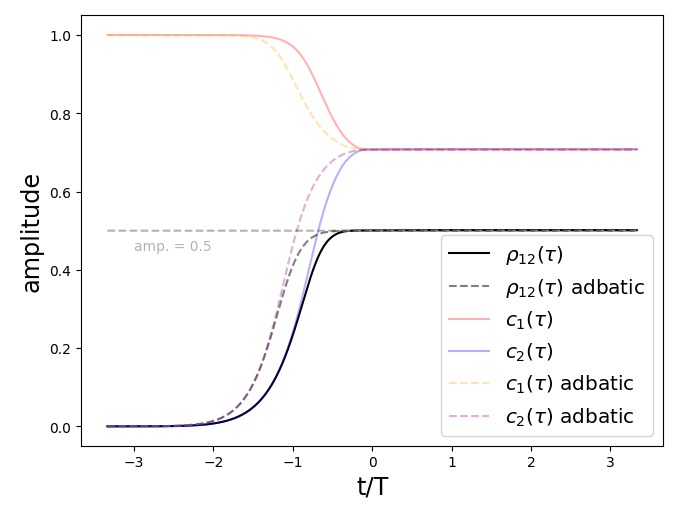
\includegraphics[scale=0.8]{542HW1/P3}
\end{center}

From the figure, we clearly see that, both $\rho_{12}(\tau)$ calculated via adiabatic approximation and calculated numerically approaches $1/2$ in the limit $\tau \to \infty$, as expected.\\

\textit{* The code for the program is attached on the next page.}

\newpage
\subsection*{Script by Jinyan Miao for P1 and P3 on Physics 542 Homework 1}
\subsection*{Script for P1}
\lstset{style=mystyle}
\lstinputlisting[language=Python]{542HW1/numericalSolveP1.py}
\hfill\break
\hfill\break
\subsection*{Script for P3}
\lstset{style=mystyle}
\lstinputlisting[language=Python]{542HW1/numericalSolveP3.py}





\chapter{}
Here we consider the field of the form 
\begin{align*}
\mathbf{E}(t) = E_0\left(\hat{\mathbf{x}}\cos(\omega t) + \hat{\mathbf{y}}\sin(\omega t) \right)\,,
\end{align*}
with $E_0\in \R$ being a constant. We define 
\begin{align*}
\mathbf{\epsilon}_{\pm} = \mp \frac{\hat{\mathbf{x}}\pm i \hat{\mathbf{y}}}{\sqrt{2}}\,.
\end{align*}
Thus we can write
\begin{align*}
\frac{E_0}{\sqrt{2}}(-\hat{\epsilon}_+ e^{-i \omega t} + \hat{\epsilon}_- e^{i \omega t}) 
&= 
\frac{E_0}{\sqrt{2}} \left( \frac{\hat{\mathbf{x}}+ i \hat{\mathbf{y}}}{\sqrt{2}}(\cos(\omega t) + i \sin(\omega t)) + \frac{\hat{\mathbf{x}}- i \hat{\mathbf{y}}}{\sqrt{2}}(\cos(\omega t) + i \sin(\omega t))\right)\\
&= 
\frac{E_0}{2} \left( (\hat{\mathbf{x}}+ i \hat{\mathbf{y}})(\cos(\omega t) - i \sin(\omega t)) + (\hat{\mathbf{x}}- i \hat{\mathbf{y}})(\cos(\omega t) + i \sin(\omega t))\right)\\
&= 
\frac{E_0}{2} \left( (\hat{\mathbf{x}}+ i \hat{\mathbf{y}})(\cos(\omega t) - i \sin(\omega t)) + (\hat{\mathbf{x}}- i \hat{\mathbf{y}})(\cos(\omega t) + i \sin(\omega t))\right)\\
&= 
\frac{E_0}{2} \left(2\cos(\omega t)\hat{\mathbf{x}}+ 2\sin(\omega t)\hat{\mathbf{y}}  \right)\\
&= 
E_0 \left(\cos(\omega t)\hat{\mathbf{x}}+ \sin(\omega t)\hat{\mathbf{y}}  \right)\\
&= \mathbf{E}(t)\,.
\end{align*}
Defining $\hat{\mathbb{I}} = |1\rangle\, \langle 1 | + |2\rangle \, \langle 2|$. Now we can compute the interaction Hamiltonian
\begin{align*}
\hat{\mathbb{I}}\hat{H}_I \hat{\mathbb{I}} = -
\frac{E_0}{\sqrt{2}}
\left(|1\rangle\, \langle 1 | + |2\rangle \, \langle 2|\right)
(-\hat{\mu}\cdot \hat{\epsilon}_+ e^{-i \omega t} + \hat{\mu}\cdot \hat{\epsilon}_- e^{i \omega t}) 
\left(|1\rangle\, \langle 1 | + |2\rangle \, \langle 2|\right)
\end{align*}
First we consider the case with $|1\rangle$ representing the level $J=0$, and $|2\rangle$ representing the level $J=1$ with $m_J = 1$. Then by assumptions, with coefficients $-2E_0/(\sqrt{2}\hbar)$ absorbed by a constant $k \in \mathbb{C}$, we have
\begin{align*}
\hat{\mathbb{I}}\hat{H}_I \hat{\mathbb{I}}
= \frac{\hbar}{2}
\left( ke^{{i \omega t}} |1\rangle\, \langle 2|+ k^*e^{-i\omega t}|2\rangle \, \langle 1|\right)
\end{align*}
Thus the full Hamiltonian reads
\begin{align*}
\mathbf{H} = \frac{\hbar}{2}\bmat{-\omega_0 & 0 \\ 0 & \omega_0} + \frac{\hbar}{2}
\bmat{0 & ke^{i\omega t}\\ k^* e^{-i \omega t} & 0} = \frac{\hbar}{2} \bmat{-\omega_0 & ke^{i\omega t} \\ k^* e^{-i\omega t} & \omega_0}
\end{align*}
Thus the Schrodinger's equation of the system reads
\begin{align}
i\hbar\, \dot{\mathbf{a}}(t) =  \frac{\hbar}{2} \bmat{-\omega_0 & ke^{i\omega t} \\ k^* e^{-i\omega t} & \omega_0}\,\mathbf{a}(t)\,.
\end{align}
In the interaction representation, $\mathbf{a}(t) = \mathbf{c}(t) \, \exp(-i\, \mathbf{E}\,t/\hbar)$, Eq.\ (4.1) becomes
\begin{align*}
i\hbar \bmat{\dot{c}_1 e^{i\omega_0 t/2} + (i\omega_0 c_1/2) e^{i \omega_0 t/2}\\
\dot{c}_2 e^{-i\omega_0 t/2} - (i\omega_0 c_2/2) e^{-i \omega_0 t/2}
}=\frac{\hbar}{2}
\bmat{-\omega_0 c_1 e^{i\omega_0 t/2} + c_2 e^{-i\omega_0 t/2} k e^{i\omega t}\\
c_1 e^{i\omega_0 t/2}k^* e^{i\omega t} + \omega_0 c_1 e^{i\omega_0 t/2}}\,,
\end{align*}
which is equivalent to the system
\begin{align}
i\hbar\, \dot{\mathbf{c}}(t) = \frac{\hbar}{2}\bmat{0 & k e^{-i\delta t} \\ k^*e^{i\delta t} & 0}\, \mathbf{c}(t)\,,
\end{align}
with the definition of detuning $\delta\coloneqq \omega_0 - \omega$. 
Comparing Eq.\ (4.1) and (4.2) to the form of Eq.\ (2.62) and (2.63) from the textbook, we see that we have arrived to the desired system of equations without using the RWA. \\

On the other hand, if $|2\rangle$ represents the level $J=1$ with $m_J = -1$ instead. Then by assumption, the interaction Hamiltonian gives
\begin{align*}
\hat{\mathbb{I}}\hat{H}_I \hat{\mathbb{I}} = \frac{\hbar}{2}\left( -ke^{-i \omega t}|1\rangle \, \langle 2| - k^* e^{i\omega t} |2\rangle\,\langle 1|\right)\,.
\end{align*}
Similar argument leads to the system
\begin{align*}
i\hbar\, \dot{\mathbf{a}}(t) = \frac{\hbar}{2}\bmat{-\omega_0 & -ke^{-i\omega t} \\ -k^* e^{i\omega t} & \omega_0}\, \mathbf{a}(t)\,,
\end{align*}
and in the interaction representation, 
\begin{align*}
i\hbar\, \dot{\mathbf{c}}(t) = \frac{\hbar}{2}\bmat{0 & -ke^{-i(\omega+\omega_0) t} \\ -k^* e^{i(\omega+\omega_0) t} & 0}\, \mathbf{c}(t)\,,
\end{align*}
suggesting that the counterrotating term (with frequency $\omega+\omega_0$) drives the transitions between the two levels. 





\end{document}


